\documentclass{article}
\usepackage[margin=1.0in]{geometry}
\usepackage[utf8]{inputenc}
\usepackage[colorlinks = true, urlcolor = blue]{hyperref}
\setlength{\parindent}{0pt}

\title{CS 6540 --- Human-Computer Interaction\\\textbf{Project 1: CITI Human Subjects Training}}
\author{ }
\date{\textbf{Due:} TBD}

\usepackage{natbib}
\usepackage{graphicx}

\begin{document}

\maketitle

\section{Summary}
The general purpose of this assignment is to complete the CITI (Collaborative Institutional Training Initiative) Social / Behavioral Research training. \\
%This gives you an introduction to ethics and related issues with human subjects research, shows you what real human subjects training looks like, and acts as functional human subjects training to participate in socio-behavioral research at the University of Utah.

\textbf{Learning Objectives:}
\begin{enumerate}
    \item Gain a basic understanding of the history leading to the creation of Institutional Review Boards.
    \item Gain a basic understanding of the definitions of \textit{research} and \textit{human subjects research.}
    \item Gain a basic understanding of the issues of \textit{respect for persons}, \textit{beneficence}, and \textit{justice}, including:
    \begin{itemize}
        \item Informed consent
        \item Confidentiality
        \item Protected populations
    \end{itemize}
    \item Become eligible to participate in (IRB-approved) Social / Behavioral research at the University of Utah.
\end{enumerate}\\

\section{To Do}
\begin{enumerate}
    \item Register an account at \href{https://about.citiprogram.org/}{https://about.citiprogram.org/}. You should make sure that your account is created as being affiliated with the University of Utah, instead of as an independent learner. The University of Utah pays for access to certain CITI modules. To be clear, you \textbf{should not need to pay anything}.
    
    \begin{figure}[h!]
    \centering
    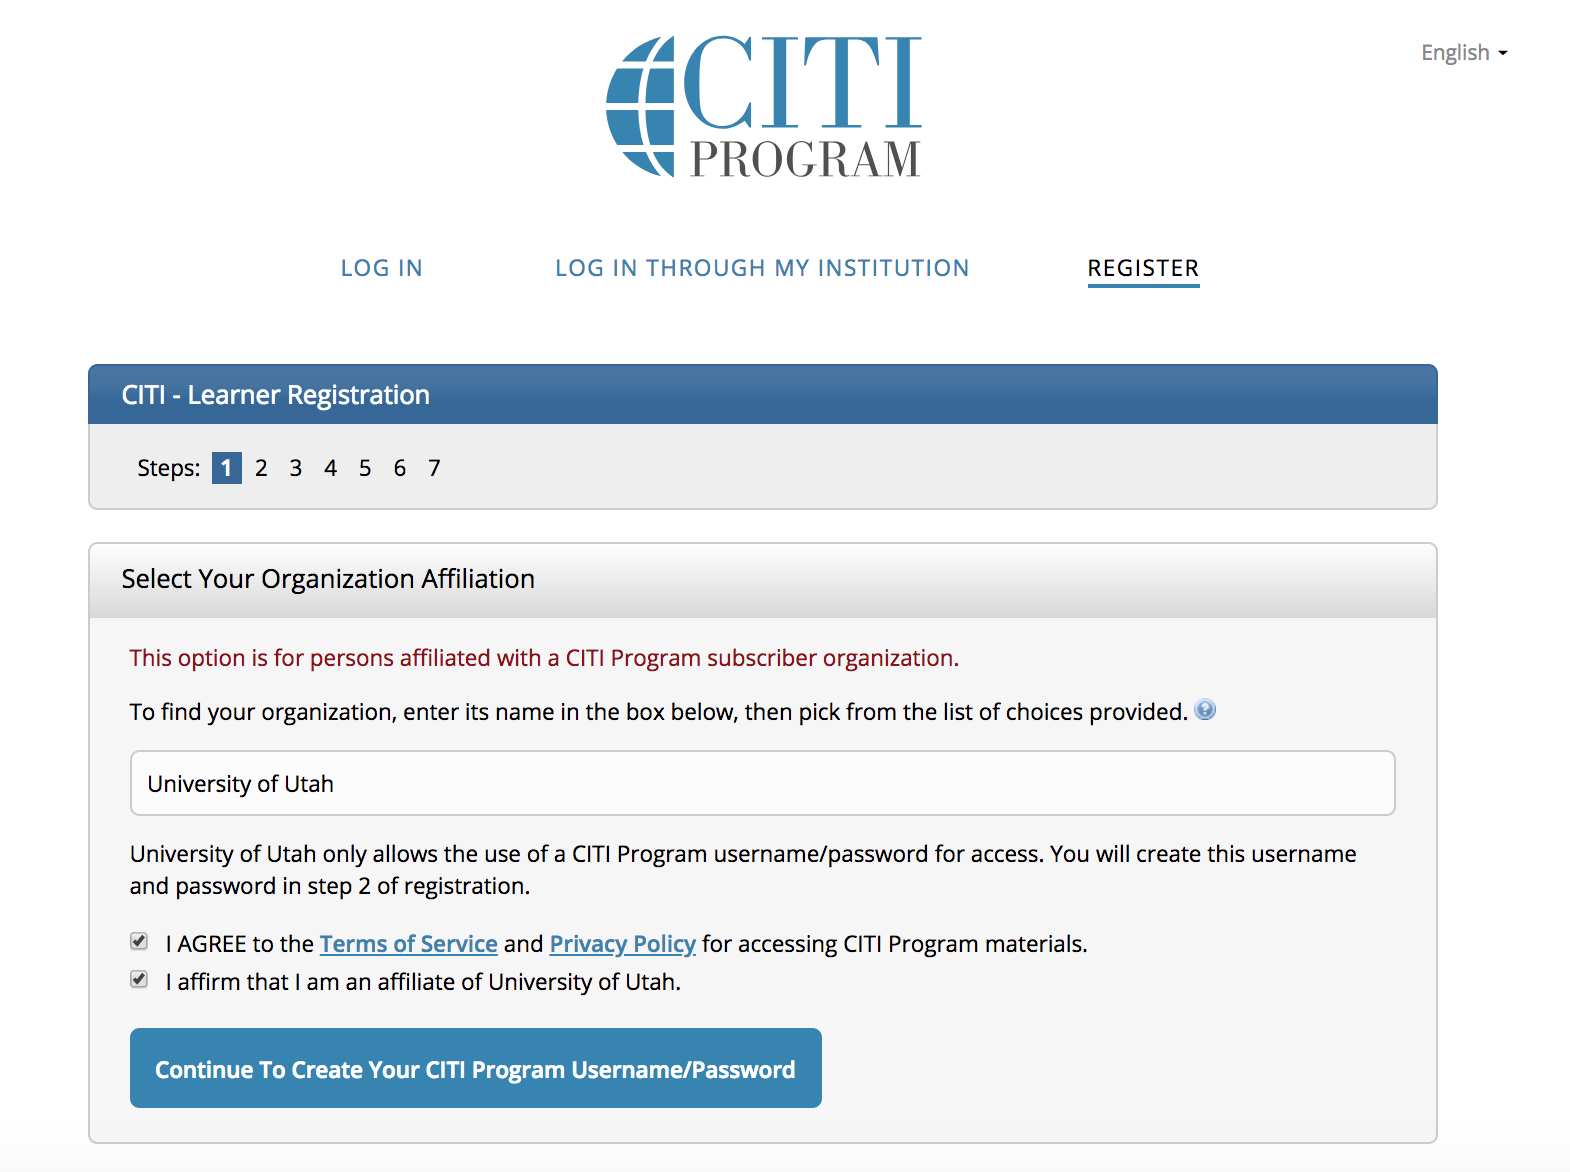
\includegraphics[scale=0.5]{CITI-registration-page}
    \caption{Register an account with CITI via the University of Utah's association with the site.}
    \end{figure}
    
    \item Go to the \textbf{Main Menu / My Courses} menu, then under \textbf{University of Utah Courses} click to \textbf{Add a Course}. Add  \textbf{Group 2: Social / Behavioral Research Investigators and Key Personnel}. You don't need to do the VA module or any other optional courses. If you have the option (you may not), don't take a refresher course - make sure that you (re)take the basic training.
    
    \item Per the instructions on the CITI site, you need to: (1) Complete all 17 required modules. (2) Achieve an average score of at least 80\% on all quizzes associated with the course’s module requirements. You cannot complete the modules until you complete the integrity assurance statement. As of creating this handout, the modules are:
    \begin{itemize}
        \item Belmont Report and Its Principles 
        \item History and Ethical Principles 
        \item Defining Research with Human Subjects 
        \item The Federal Regulations
        \item Assessing Risk
        \item Informed Consent
        \item Privacy and Confidentiality
        \item Research with Prisoners
        \item Research with Children
        \item Research in Public Elementary and Secondary Schools \item International Research
        \item Students in Research
        \item Internet-Based Research
        \item Research and HIPAA Privacy Protections
        \item Conflicts of Interest in Human Subjects Research
        \item Unanticipated Problems and Reporting Requirements in Social and Behavioral Research
        \item University of Utah
    \end{itemize}
    Module lengths vary. The modules consist of reading and a quiz.
\end{enumerate}


\section{To Turn In}
Once you've completed the training, click on \textbf{View-Print-Share} to access the report of your completion. Turn in the PDF to Canvas.

    \begin{figure}[h!]
    \centering
    
\includegraphics[scale=1.0]{CITI-completion-report}
    \caption{Your completion PDF should look something like this.}
    \end{figure}

\end{document}
